\chapter*{Tutorial Pembuatan Aplikasi Oracle Apex}

\begin{enumerate}
	\item Buka Website Oracle Apex,  https://apex.oracle.com

	\item Lengkapi Request a Workspaces seperti dibawah ini 
	\begin{figure} [!htbp]
	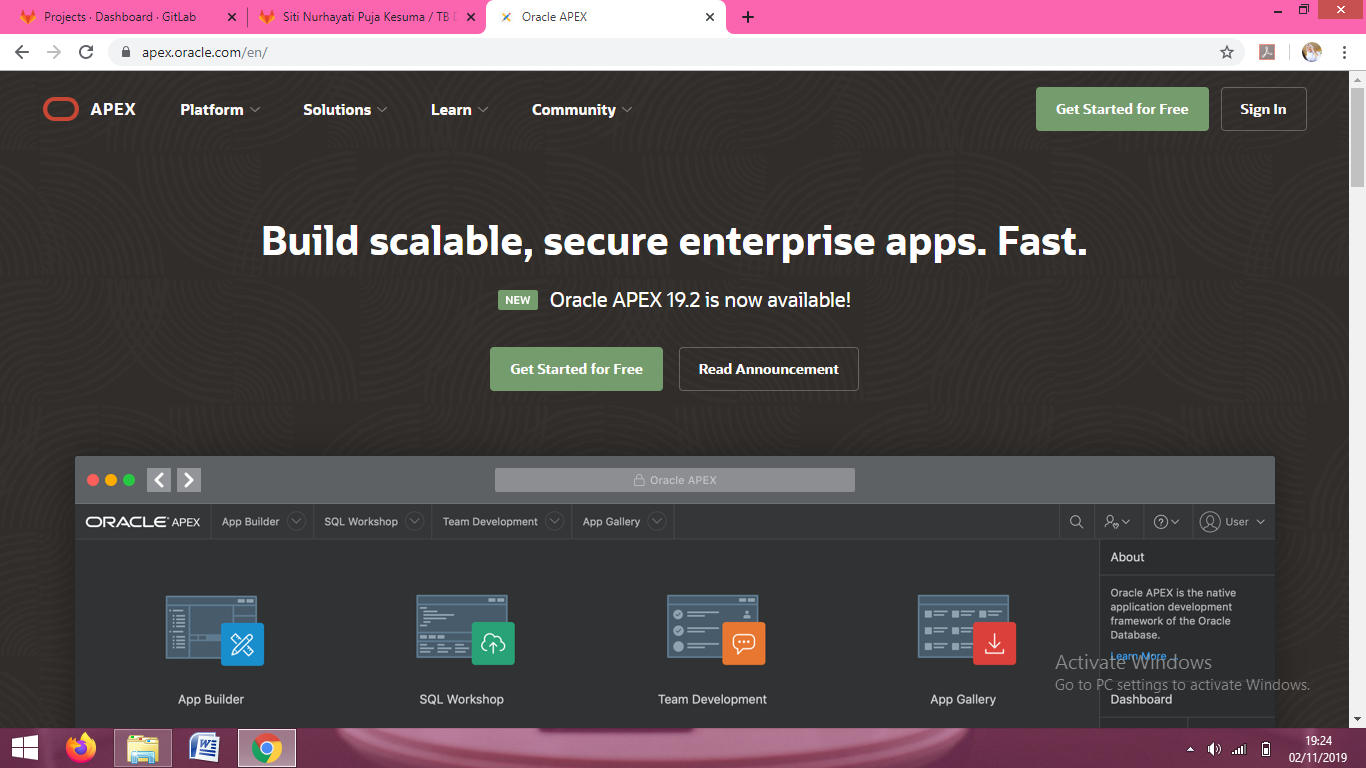
\includegraphics[scale=0.2]{section/gambar/a.png}
	\centering
	\end{figure}

	\item Mengisi Justification
	\begin{figure} [!htbp]
	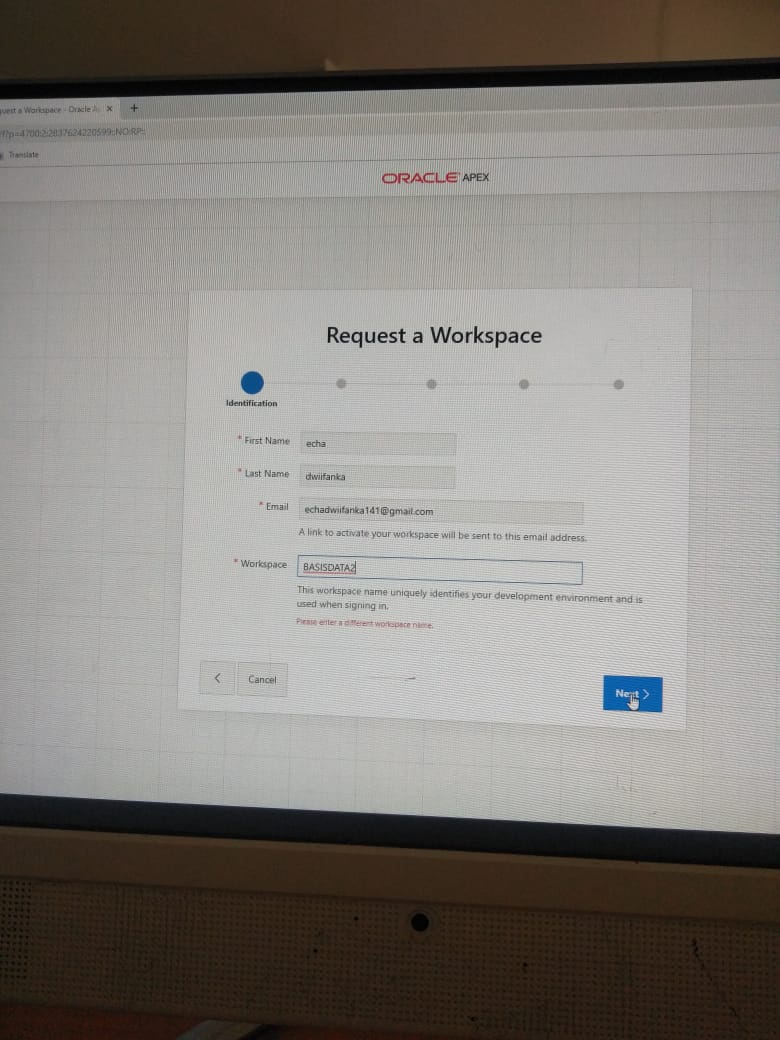
\includegraphics[scale=0.2]{section/gambar/1.jpeg}
	\centering
	\end{figure}
	
	\item Dan submit Request
	\begin{figure} [!htbp]
	\includegraphics[]{}
	\centering
	\end{figure}
	
	\item Dan akan mendapatkan email seperti dibawah ini lalu klik create workspaces 
	\begin{figure} [!htbp]
	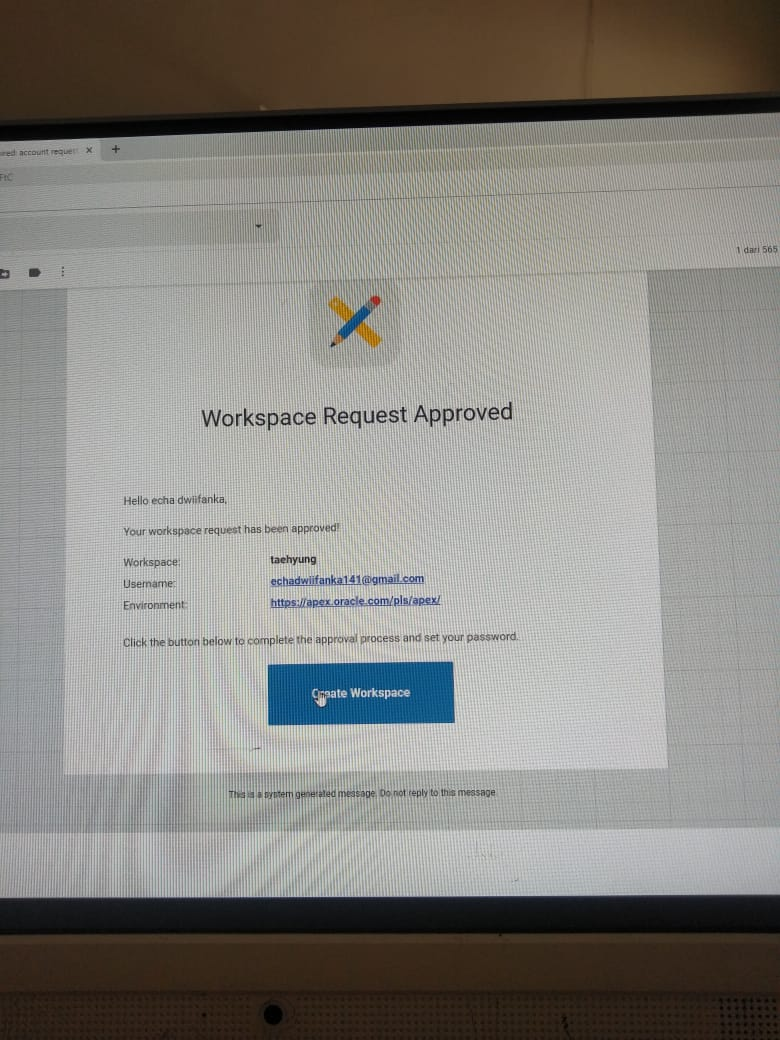
\includegraphics[scale=0.2]{section/gambar/5.jpeg}
	\centering
	\end{figure}
	
	\item Workspace Succesfully akan muncul seperti gambar dibawah ini dan kllik continue to sign in screen
	\begin{figure} [!htbp]
	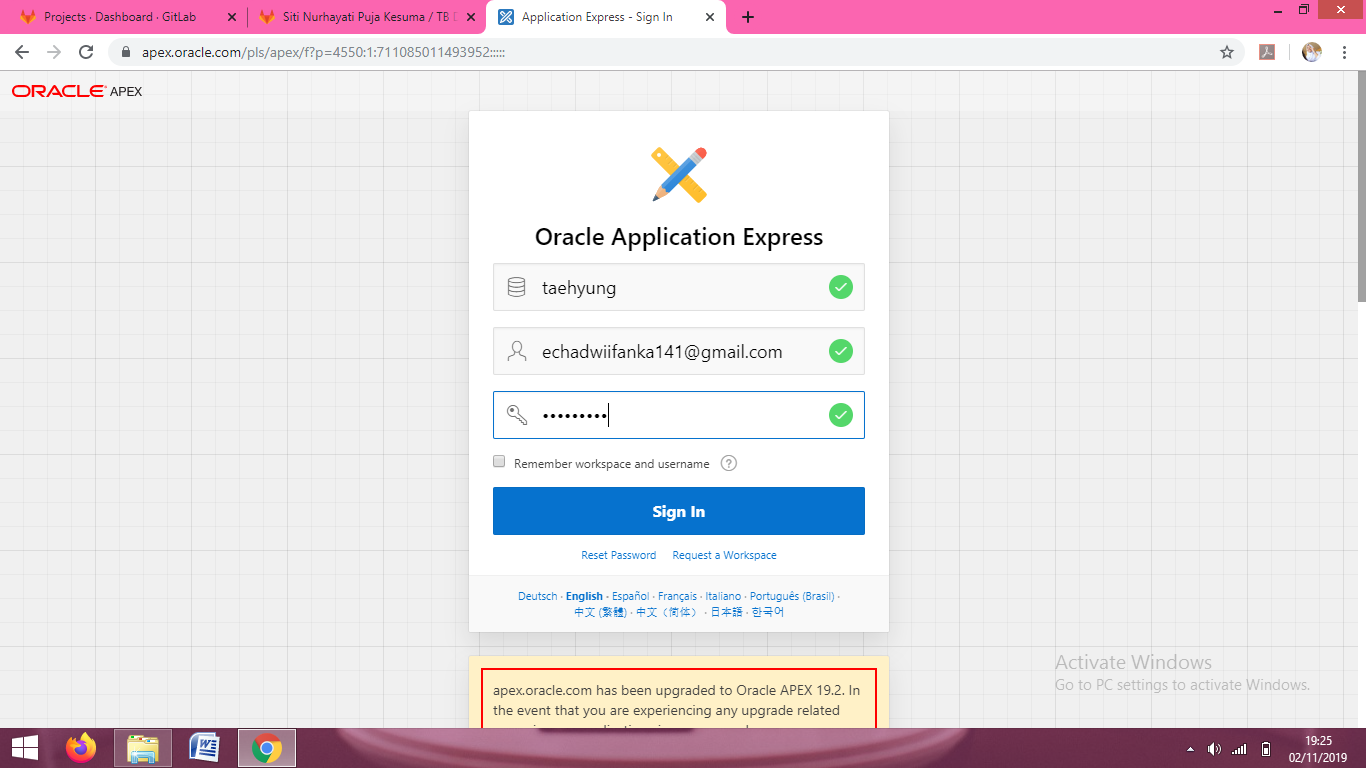
\includegraphics[scale=0.2]{section/gambar/b.png}
	\centering
	\end{figure}
	
	\item dan pilih App Builder
	\begin{figure} [!htbp]
	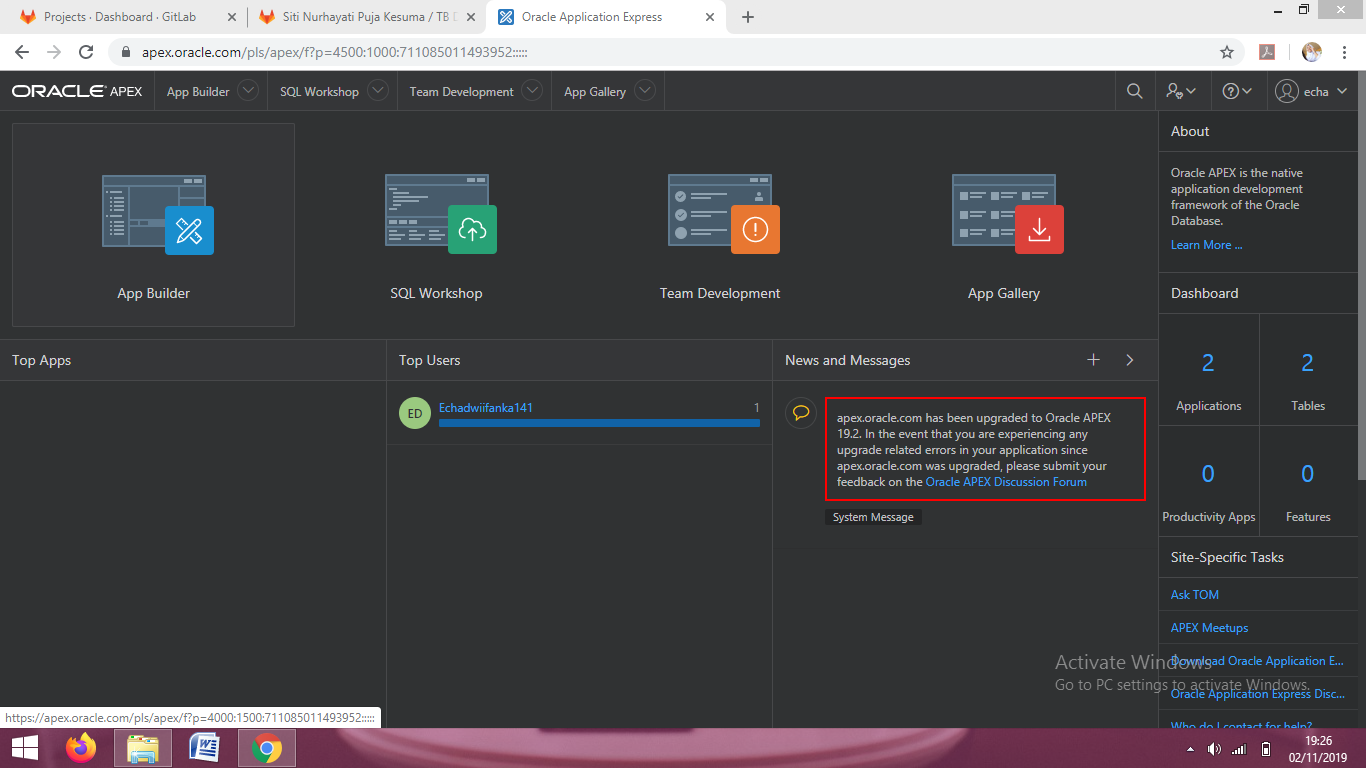
\includegraphics[scale=0.2]{section/gambar/c.png}
	\centering
	\end{figure}
	
	\item Lalu pilih create yang seperti digambar 
	\begin{figure} [!htbp]
	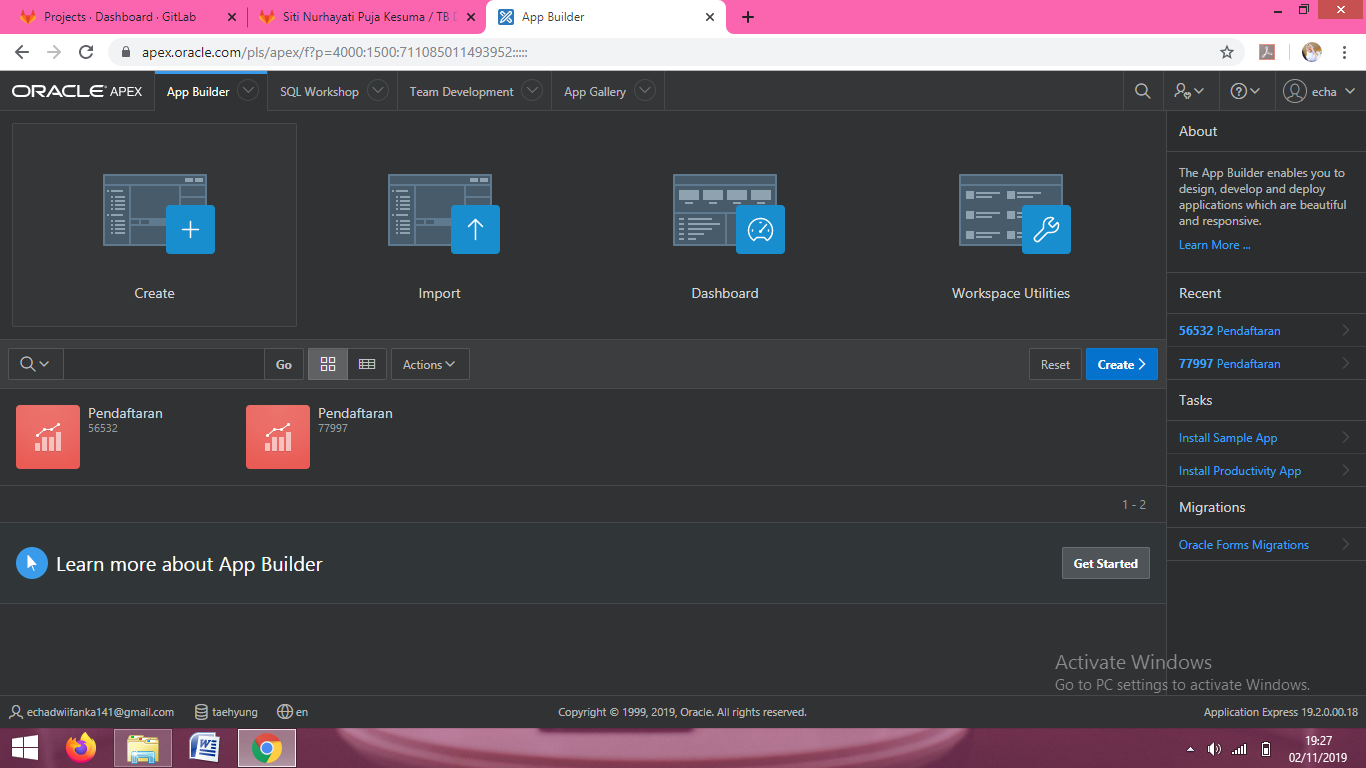
\includegraphics[scale=0.2]{section/gambar/d.png}
	\centering
	\end{figure}
	
	\item Lalu siapkan file yang akan di import ke exelworkbook atau CSV seperti yang ada digambar 
	\begin{figure} [!htbp]
	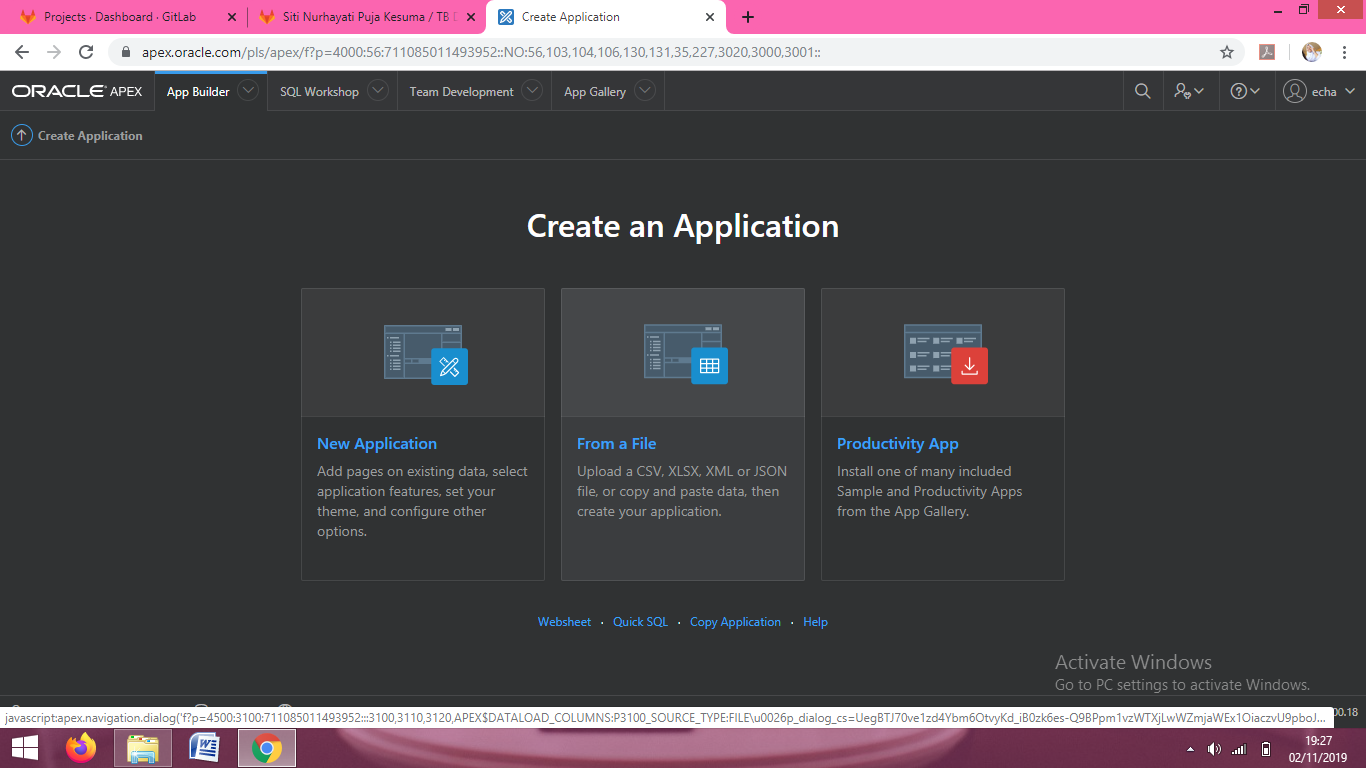
\includegraphics[scale=0.2]{section/gambar/e.png}
	\centering
	\end{figure}

\item lalu pilih From file 
	\begin{figure} [!htbp]
	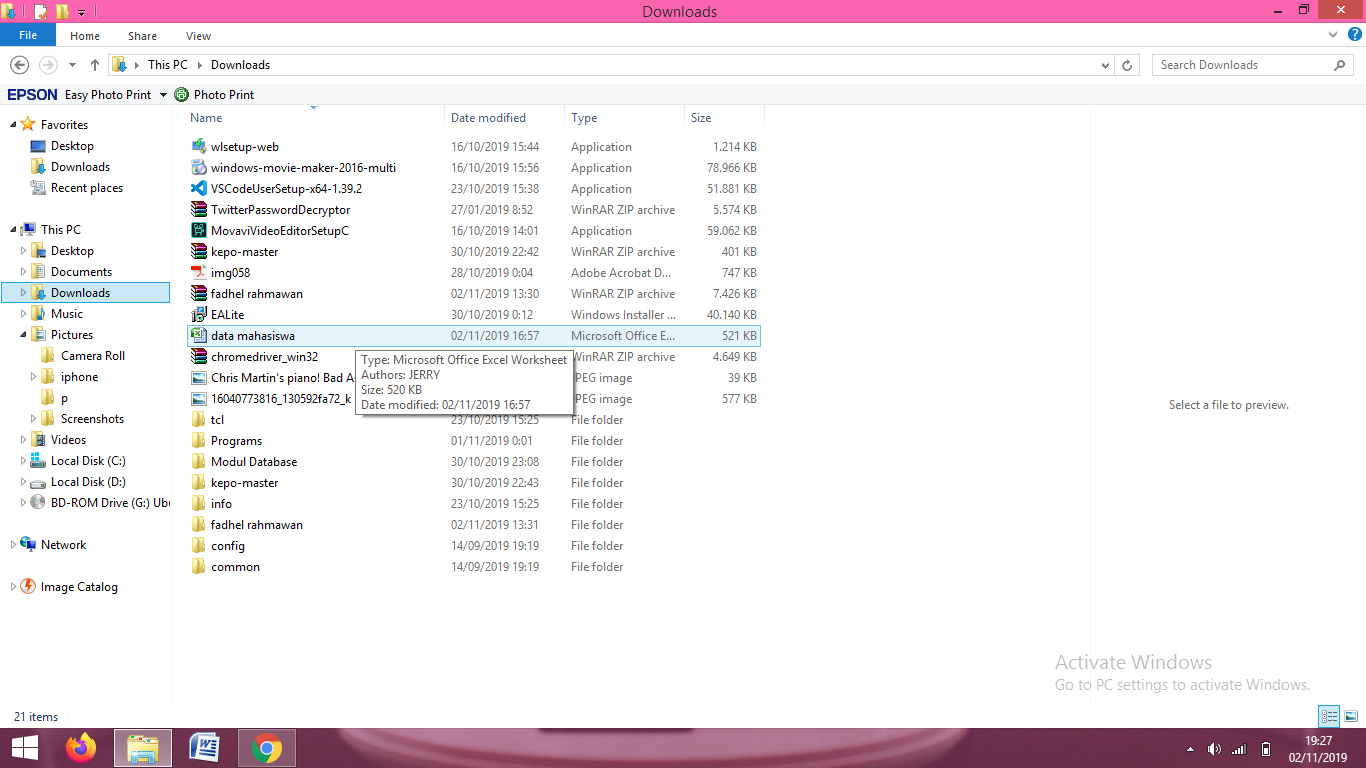
\includegraphics[scale=0.2]{section/gambar/f.png}
	\centering
	\end{figure}
	
	\item lalu isi form seperti digambar 
	\begin{figure} [!htbp]
	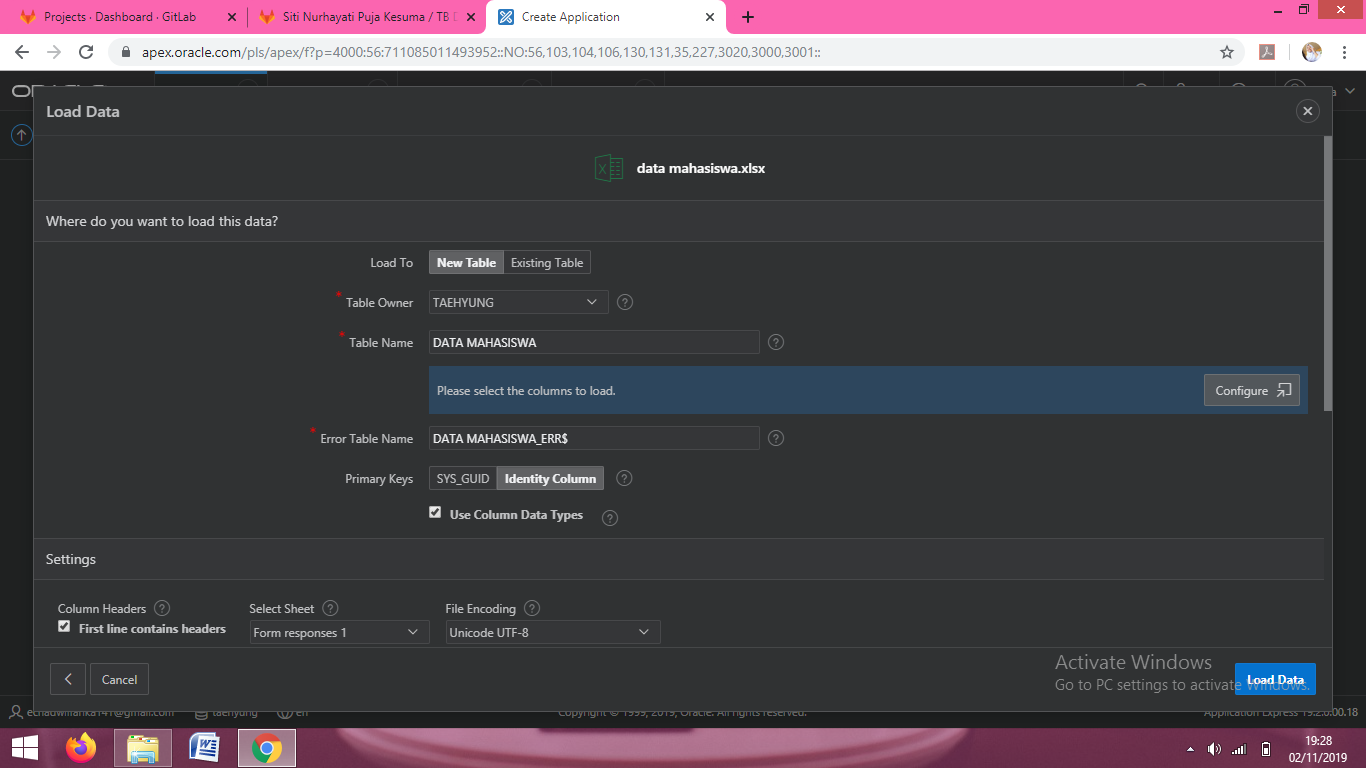
\includegraphics[scale=0.2]{section/gambar/g.png}
	\centering
	\end{figure}
	
	
	\item Dan akan berhasil seperti dibawah 
	\begin{figure} [!htbp]
	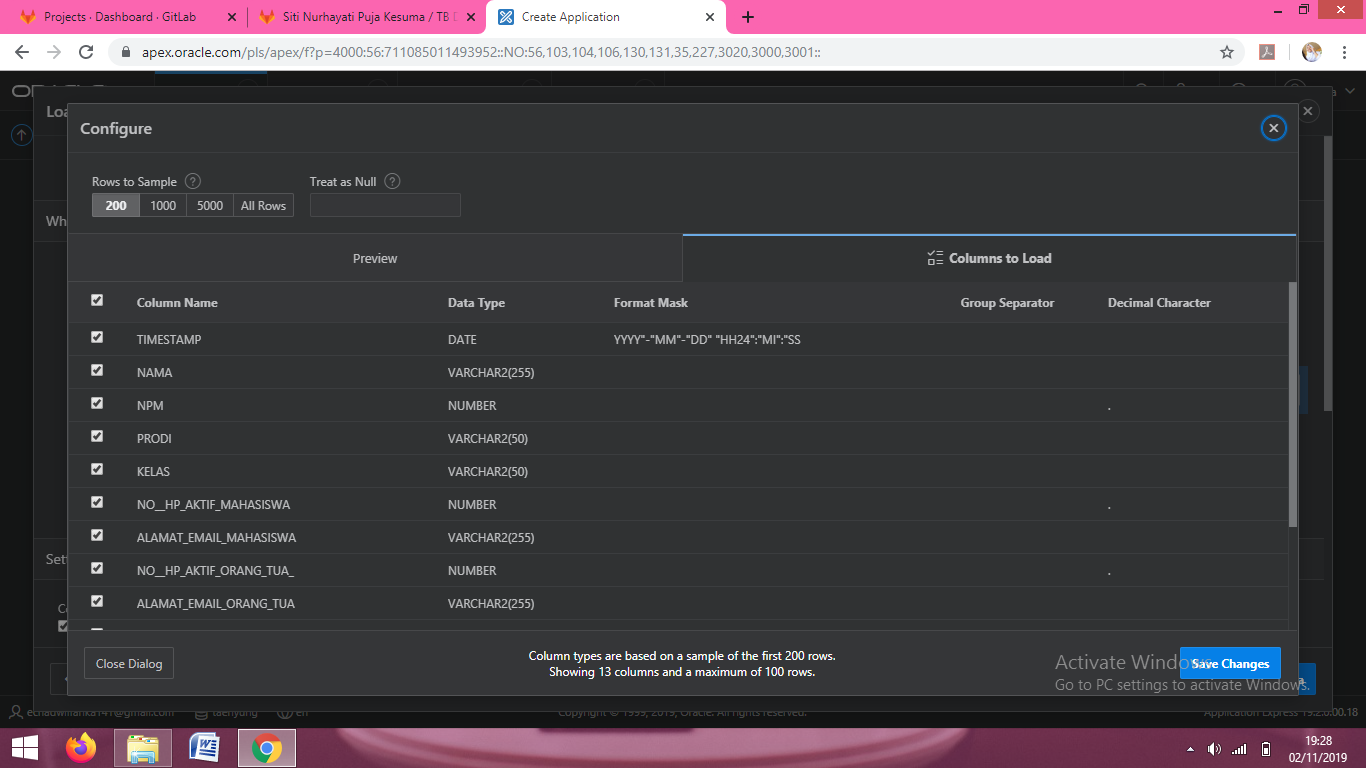
\includegraphics[scale=0.2]{section/gambar/h.png}
	\centering
	\end{figure}
	
	\item Lalu lanjutkan dengan membuat create aplication
	\begin{figure} [!htbp]
	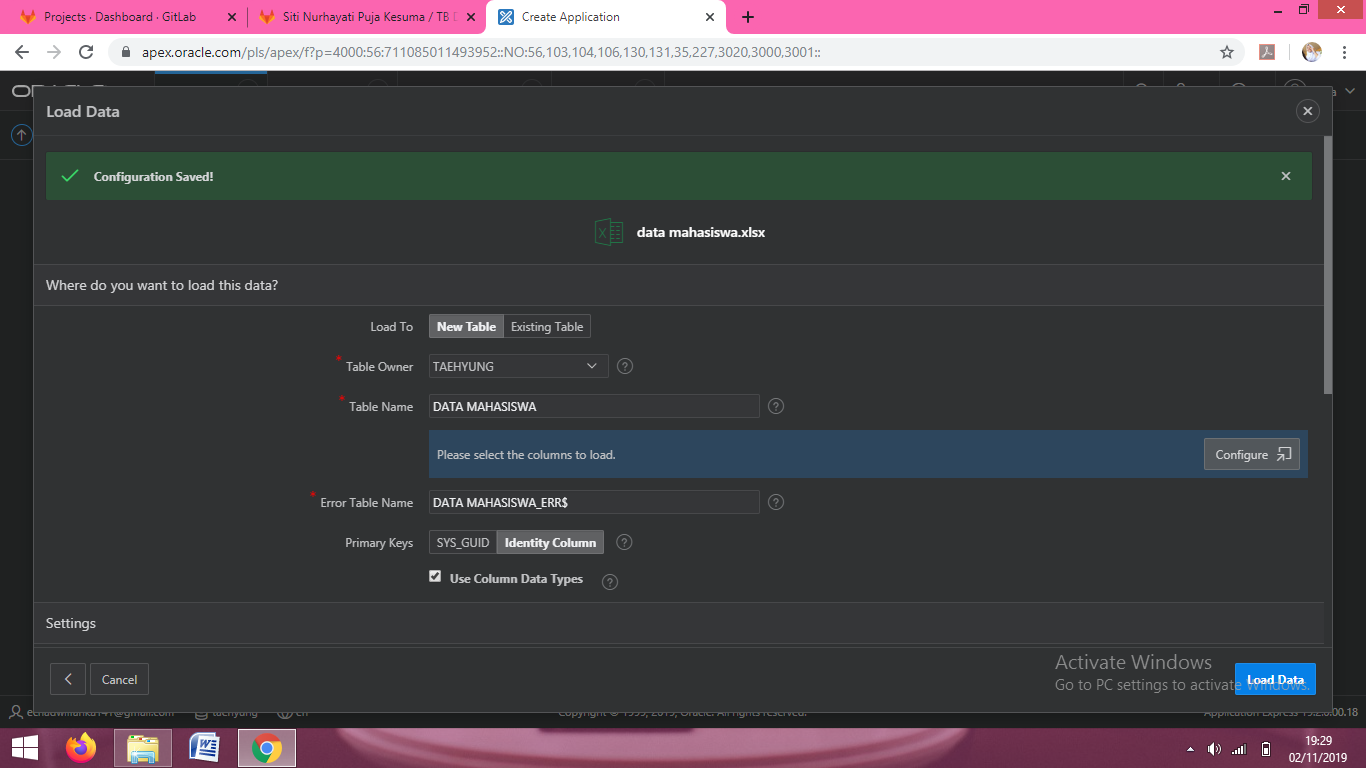
\includegraphics[scale=0.2]{section/gambar/i.png}
	\centering
	\end{figure}
	\begin{figure} [!htbp]
	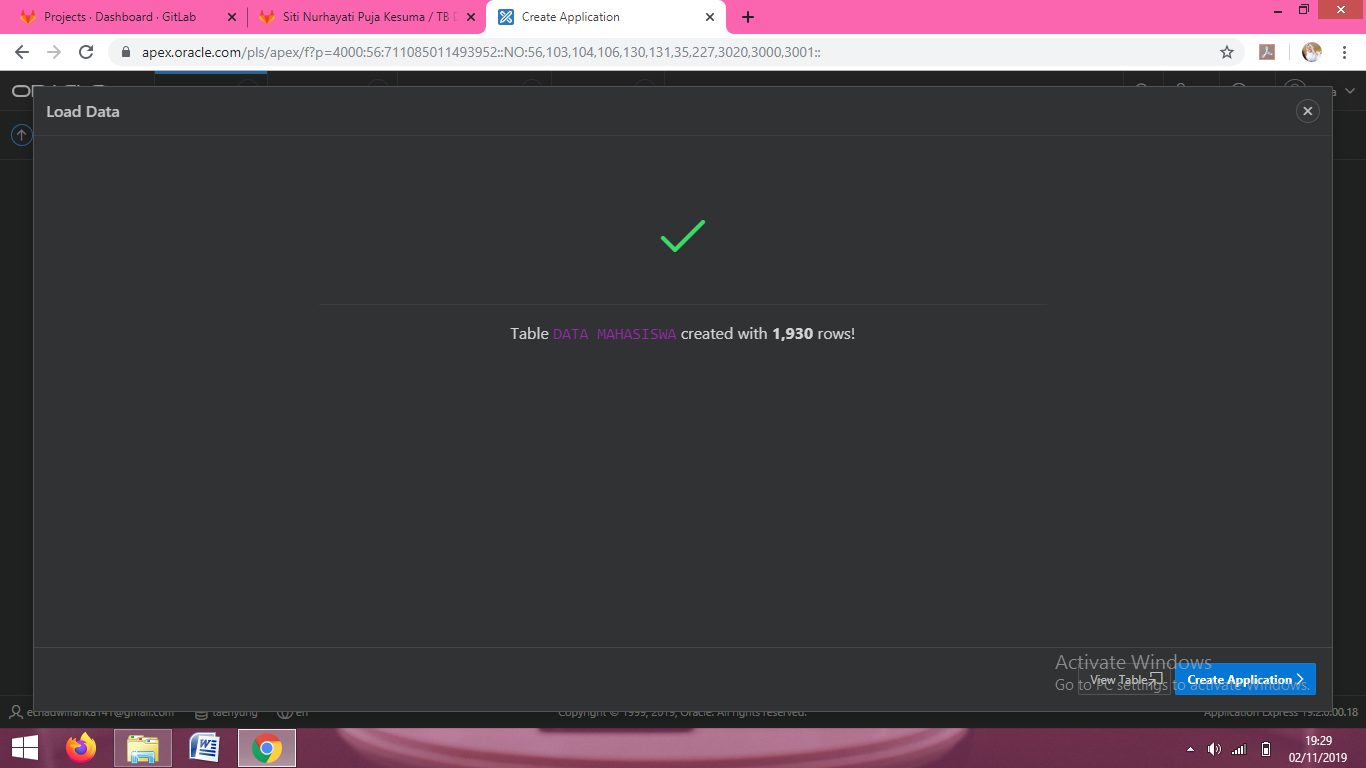
\includegraphics[scale=0.2]{section/gambar/j.png}
	\centering
	\end{figure}
	
	\begin{figure} [!htbp]
	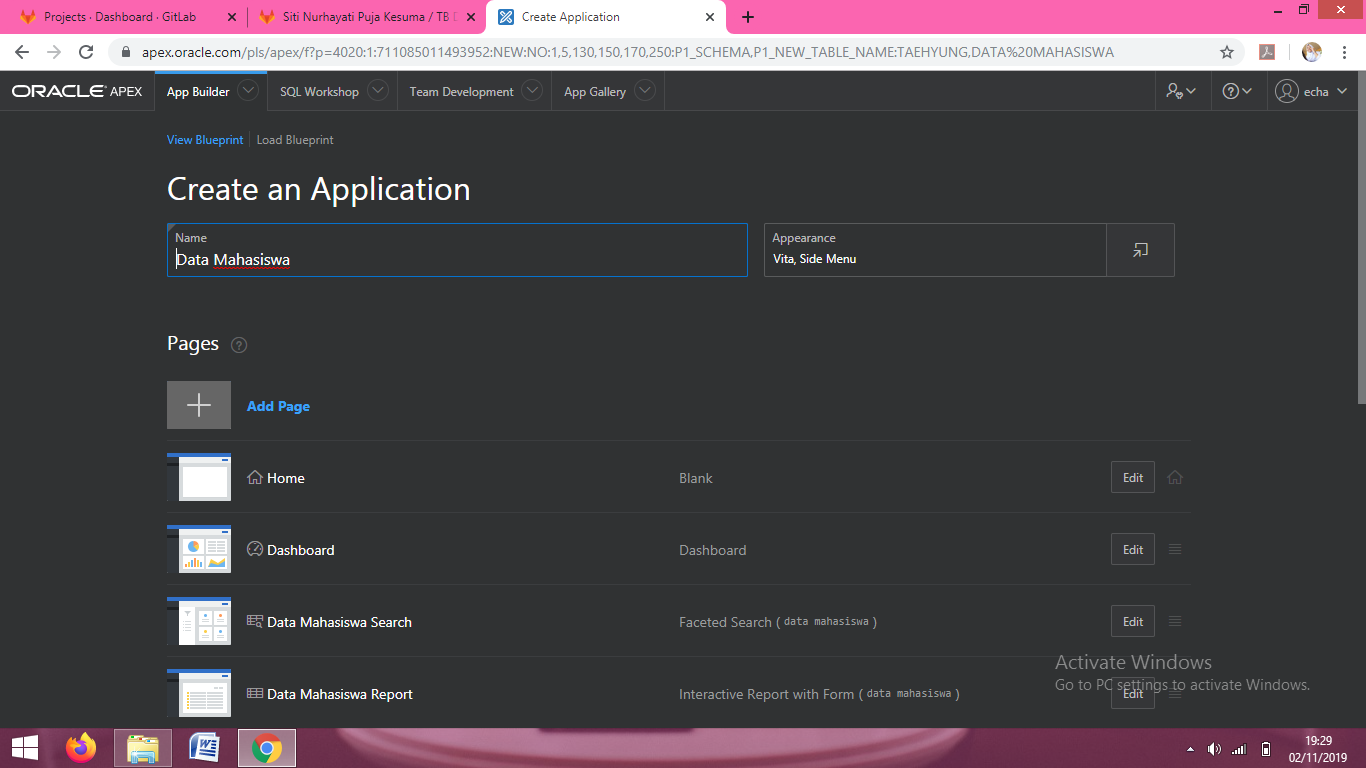
\includegraphics[scale=0.2]{section/gambar/k.png}
	\centering
	\end{figure}
	
	\begin{figure} [!htbp]
	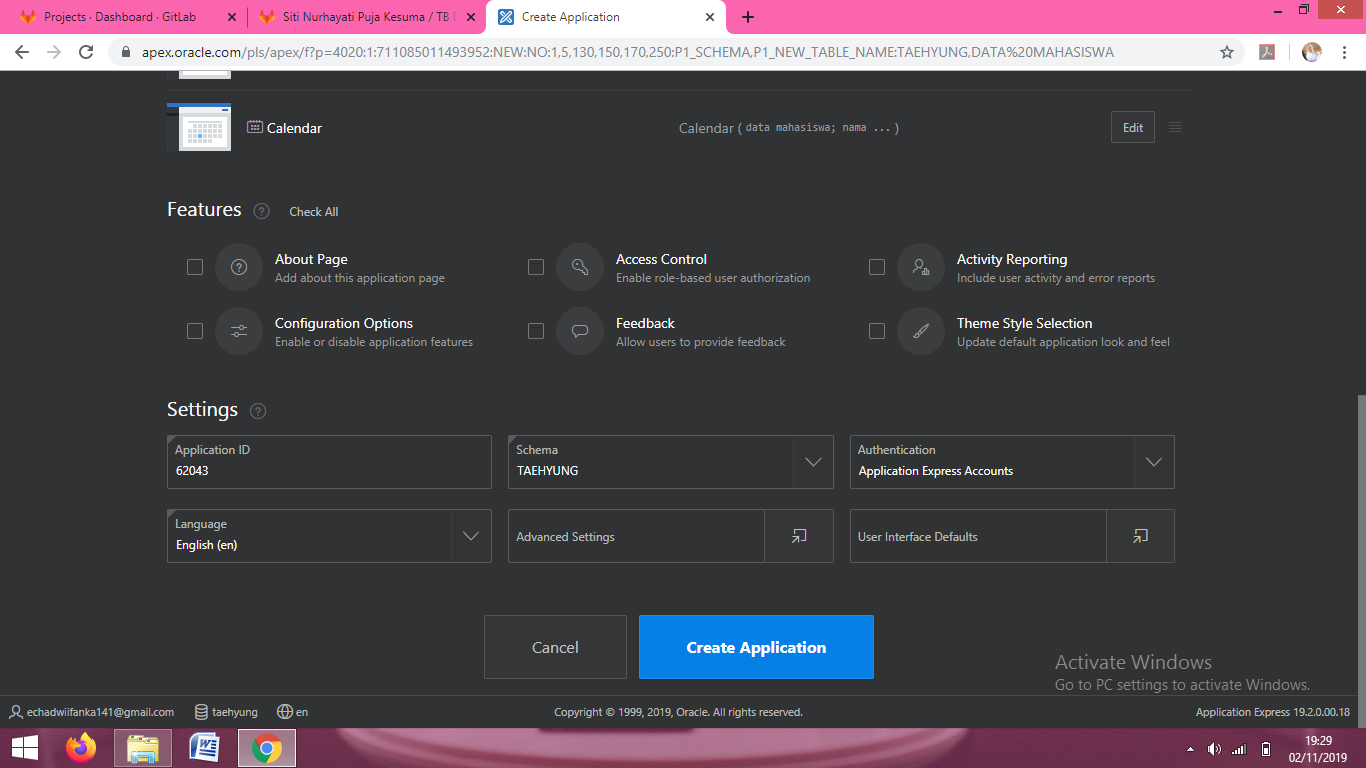
\includegraphics[scale=0.2]{section/gambar/l.png}
	\centering
	\end{figure}
	
	\begin{figure} [!htbp]
	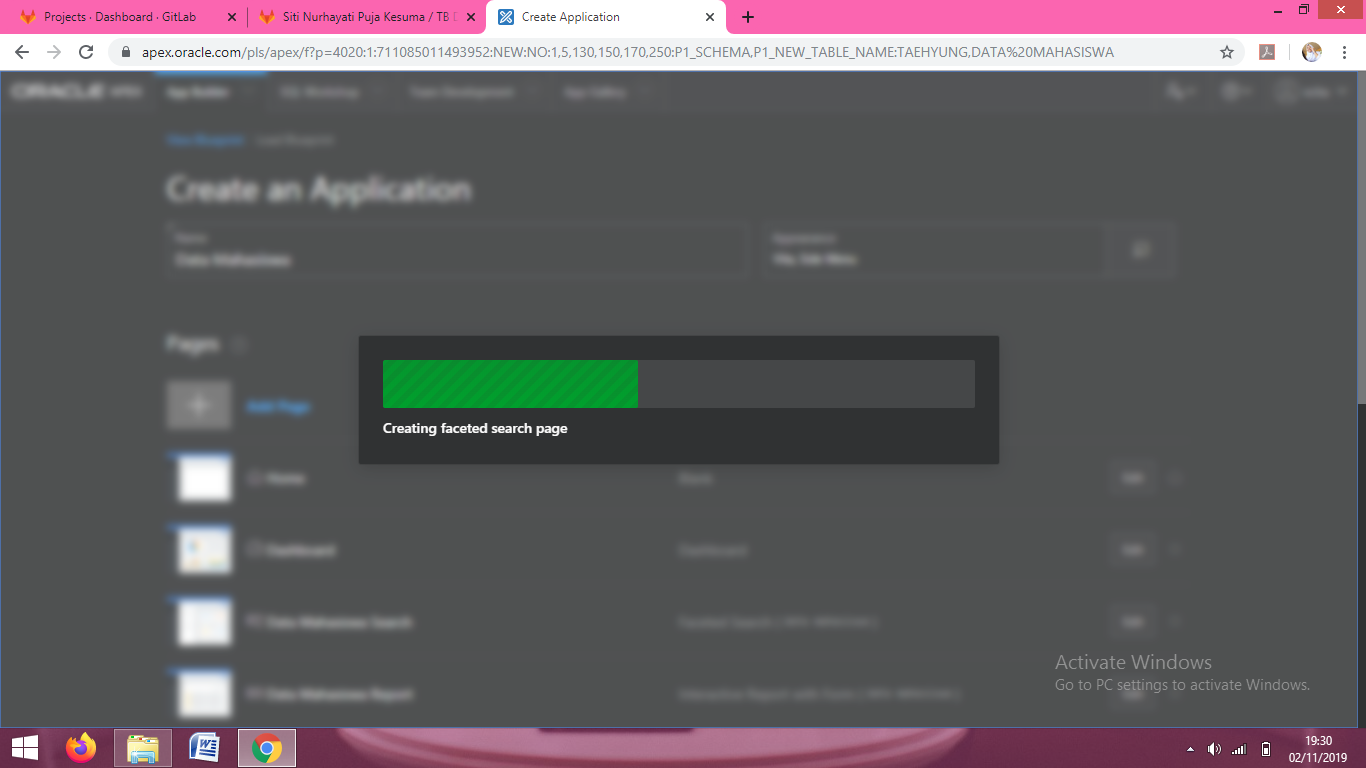
\includegraphics[scale=0.2]{section/gambar/m.png}
	\centering
	\end{figure}
	
	\item lalu klik run-aplication
	\begin{figure} [!htbp]
	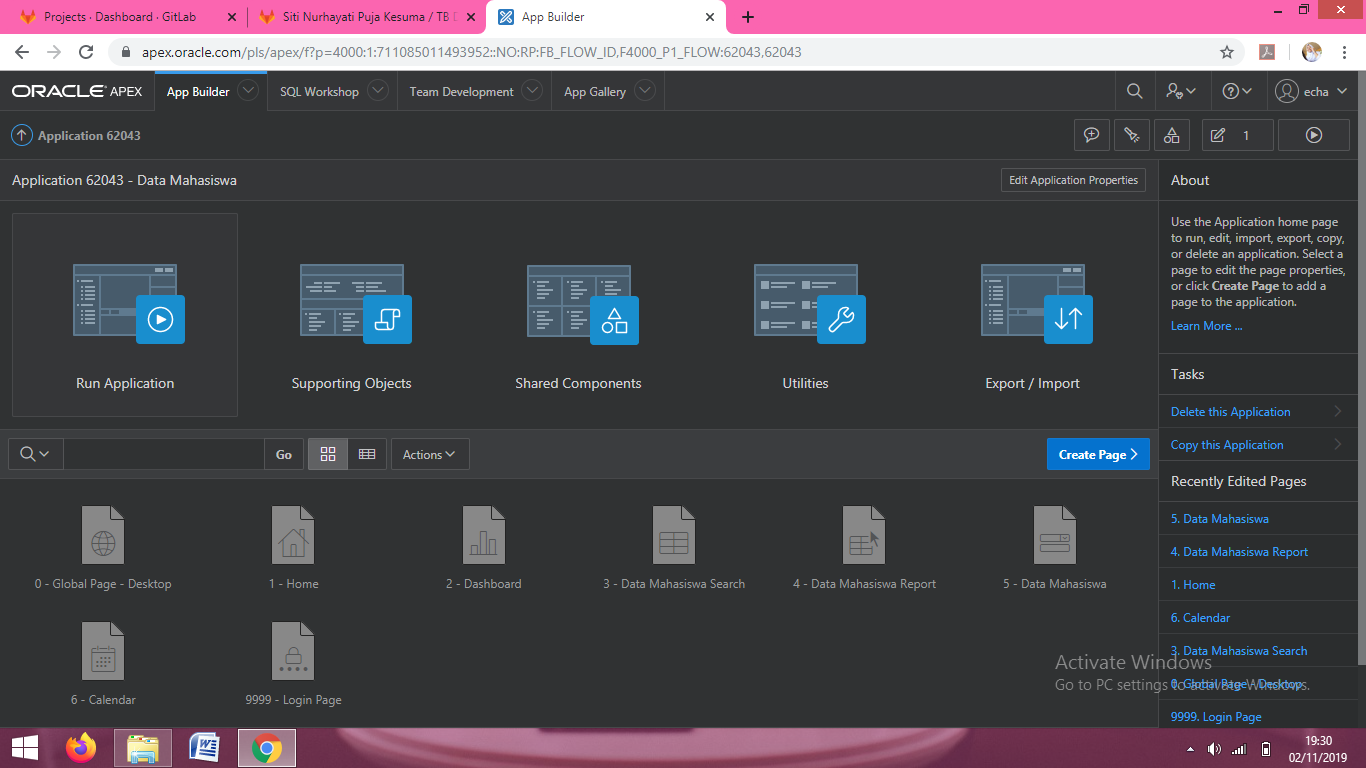
\includegraphics[scale=0.2]{section/gambar/n.png}
	\centering
	\end{figure}
	
	\item dan login ulang kembali 
	\begin{figure} [!htbp]
	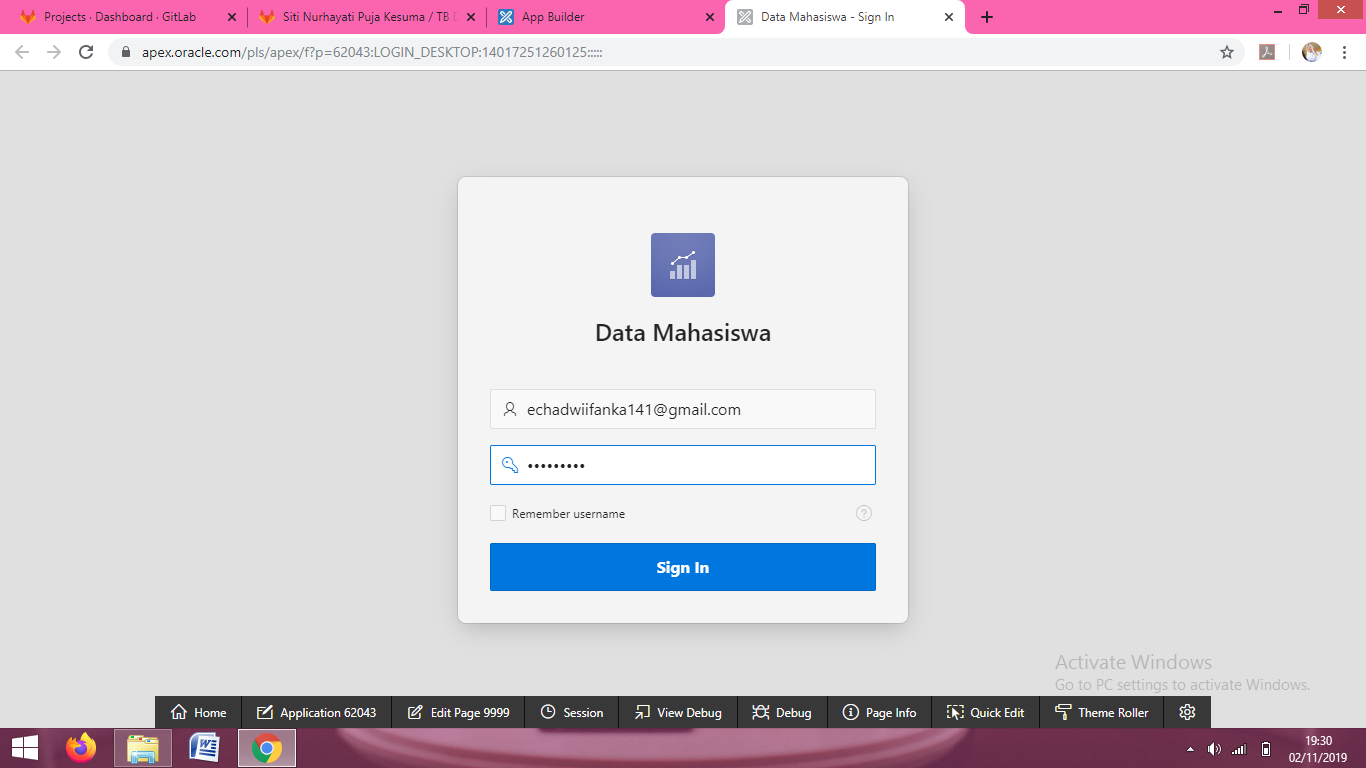
\includegraphics[scale=0.2]{section/gambar/o.png}
	\centering
	\end{figure}
	
	\item dan akan keluar seperti dibawah ini
	\begin{figure} [!htbp]
	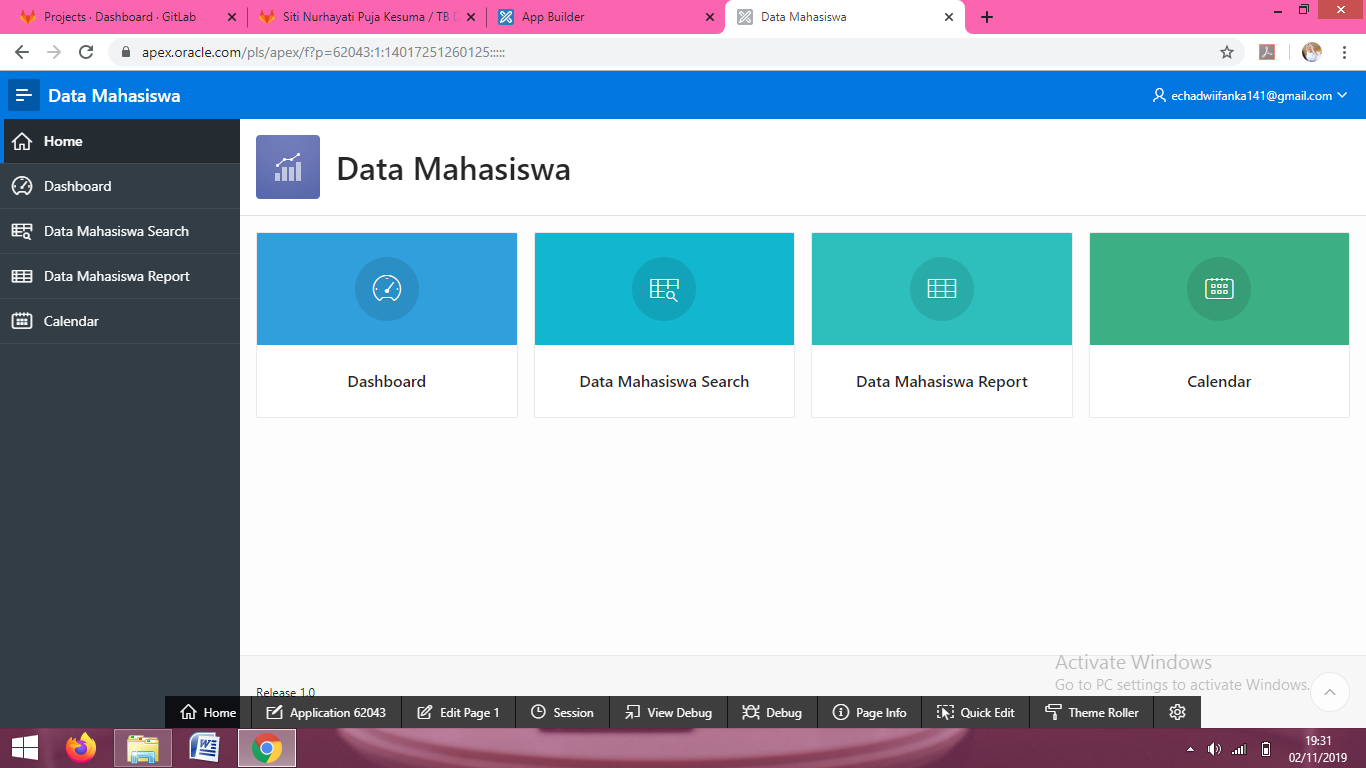
\includegraphics[scale=0.2]{section/gambar/p.png}
	\centering
	\end{figure}
	
	\begin{figure} [!htbp]
	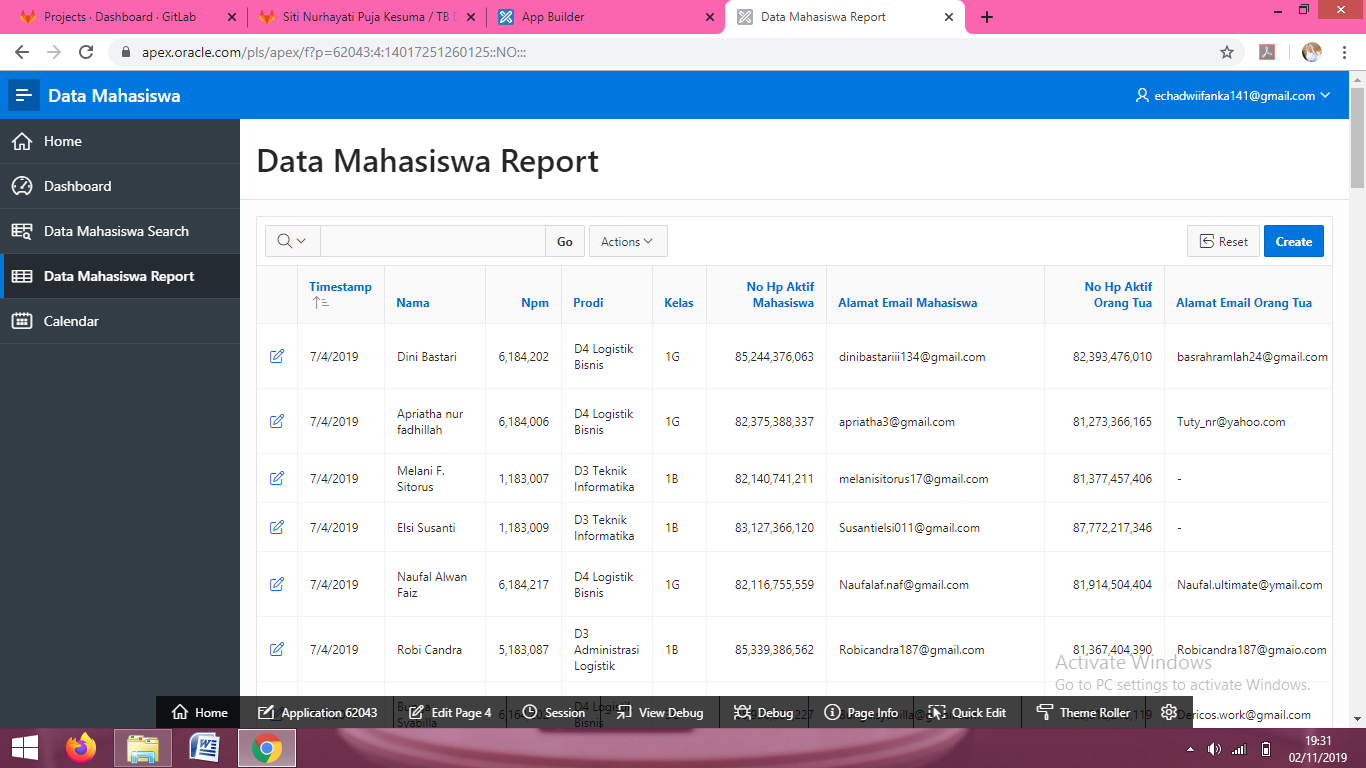
\includegraphics[scale=0.2]{section/gambar/q.png}
	\centering
	\end{figure}
	
	\begin{enumerate}
	    \item[1.]workspaces : taehyung
	    \item[2.] password : Echadwi14
	    \item[3.] user : echadwiifanka141@gmail.com
	\end{enumerate}
\end{enumerate}
